\documentclass[conference]{IEEEtran}
\IEEEoverridecommandlockouts
\usepackage[utf8]{inputenc}
\usepackage{cite}
\usepackage{amsmath,amssymb,amsfonts}
\usepackage{algorithmic}
\usepackage{graphicx}
\usepackage{textcomp}
\usepackage{xcolor}
\def\BibTeX{{\rm B\kern-.05em{\sc i\kern-.025em b}\kern-.08em
    T\kern-.1667em\lower.7ex\hbox{E}\kern-.125emX}}
\begin{document}

\title{Interpretable Healthcare Cost Prediction Using XGBoost with Dual Explainable AI Framework}

\author{\IEEEauthorblockN{Ammar Pavel Zamora Siregar}
\IEEEauthorblockA{\textit{School of Informatics}\\
\textit{Universitas Telkom}\\
Bandung, Indonesia\\
ammarpvl@student.telkomuniversity.ac.id}
\and
\IEEEauthorblockN{Achmad Udin Zailani}
\IEEEauthorblockA{\textit{School of Informatics}\\
\textit{Universitas Telkom}\\
Bandung, Indonesia\\
achmadudinzailani@telkomuniversity.ac.id}
\and
\IEEEauthorblockN{Nurul Ilmi}
\IEEEauthorblockA{\textit{School of Informatics}\\
\textit{Universitas Telkom}\\
Bandung, Indonesia\\
nurulilmi@telkomuniversity.ac.id}
}

\maketitle

\begin{abstract}
Transparansi biaya pengobatan merupakan kebutuhan kritis bagi pemberdayaan pasien dalam pengambilan keputusan perawatan kesehatan. Studi menunjukkan 92\% pasien menginginkan estimasi biaya pengobatan sebelum perawatan, namun informasi ini jarang tersedia dengan akurat. Ketidakpastian biaya menyebabkan 47\% penduduk dewasa AS mengalami kesulitan membayar biaya pengobatan dan 41\% memiliki utang medis. Penelitian ini mengimplementasikan algoritma XGBoost untuk prediksi biaya pengobatan pasien menggunakan dataset Kaggle Insurance Cost (1338 records, 7 fitur: age, sex, BMI, children, smoker, region, charges). XGBoost dipilih karena kemampuannya dalam menangani interaksi fitur kompleks dan integrasi optimal dengan teknik Explainable AI. Implementasi SHAP (SHapley Additive exPlanations) dan LIME (Local Interpretable Model-agnostic Explanations) dilakukan untuk memastikan transparansi dan interpretabilitas model. Linear Regression digunakan sebagai baseline untuk menunjukkan peningkatan performa. Framework patient-centric dikembangkan untuk menyajikan prediksi biaya pengobatan dengan penjelasan yang dapat dipahami pasien. Model XGBoost mencapai akurasi prediksi tinggi ($R^2 = 0.8770$) dengan tetap mempertahankan interpretabilitas melalui XAI. Implementasi SHAP memberikan penjelasan global dan lokal yang konsisten, sementara LIME menawarkan interpretasi cepat untuk aplikasi real-time. Framework yang dikembangkan menghasilkan dashboard interaktif yang memungkinkan pasien memahami faktor-faktor yang mempengaruhi biaya pengobatan mereka. Penelitian ini berkontribusi pada pengembangan sistem prediksi biaya pengobatan yang tidak hanya akurat tetapi juga transparan dan dapat dipahami pasien. Integrasi XGBoost dengan XAI menciptakan keseimbangan antara performa prediktif dan interpretabilitas, mendukung pasien dalam membuat keputusan kesehatan yang lebih informed. Metodologi yang dikembangkan memiliki potensi adaptasi untuk konteks sistem kesehatan Indonesia.
\end{abstract}

\begin{IEEEkeywords}
XGBoost, Explainable AI, SHAP, LIME, Healthcare Cost Prediction, Patient Empowerment
\end{IEEEkeywords}

\section{Introduction}
Healthcare cost transparency remains a critical challenge globally. In the United States, 47\% of adults struggle to pay medical bills and 41\% carry medical debt \cite{kff2024}. Despite 92\% of patients desiring out-of-pocket cost estimates before treatment \cite{sagi2024}, such information is rarely available with accuracy. This opacity not only creates financial burden but impairs healthcare decision-making quality.

Traditional statistical methods for cost prediction, such as linear regression, achieve limited accuracy ($R^2 = 0.75$) \cite{susilo2024} when modeling complex, non-linear relationships between demographic factors, lifestyle behaviors, and healthcare costs. Machine learning models like XGBoost offer superior predictive performance but suffer from interpretability challenges---a critical issue in healthcare where algorithmic decisions significantly impact patient lives and where regulations like GDPR mandate ``right to explanation'' \cite{lundberg2017}.

This paper addresses the gap between prediction accuracy and interpretability by developing an XGBoost ensemble model integrated with dual Explainable AI (XAI) techniques: SHAP (SHapley Additive exPlanations) for global model understanding and LIME (Local Interpretable Model-agnostic Explanations) for patient-facing real-time explanations. Our contributions are:

\begin{itemize}
\item \textbf{Methodological}: Domain-informed preprocessing with WHO medical standards, systematic optimization framework achieving $R^2 = 0.8770$, and dual XAI integration demonstrating SHAP-LIME complementarity.

\item \textbf{Empirical}: Quantification of smoking impact (280\% cost increase), BMI-smoking synergy (370\% for obese smokers), and 100\% correlation between top 5\% high-cost cases and smoking status.

\item \textbf{Practical}: Patient empowerment framework with quantified savings estimates (\$8,000 smoking cessation, \$45,200 combined interventions) and production-ready model with real-time explanation capability (8 seconds per patient).
\end{itemize}

\section{Related Work}

\subsection{XGBoost in Healthcare Cost Prediction}
Zhang et al. \cite{zhang2025} demonstrated XGBoost superiority in hospital patient volume prediction ($R^2 = 0.89$), highlighting its capability to capture temporal patterns and complex feature interactions. Boddapati \cite{boddapati2023} achieved $R^2 = 0.8681$ on health insurance cost prediction through hyperparameter optimization, identifying age and BMI as top predictors. Our work extends these findings by incorporating medical domain knowledge in feature engineering and achieving comparable performance ($R^2 = 0.8770$) on a smaller dataset through ensemble stacking.

\subsection{Explainable AI in Healthcare}
Orji and Ukwandu \cite{orji2024} integrated SHAP with XGBoost for medical insurance prediction, achieving 86.47\% $R^2$ and demonstrating that SHAP TreeExplainer reduces computation time by 85\% compared to KernelExplainer. Xu et al. \cite{xu2024} showed XGBoost-SHAP combination improved clinical decision-making accuracy by 23\% through waterfall plots and force plots.

Ahmed et al. \cite{ahmed2025} compared SHAP and LIME for healthcare predictions, finding SHAP provides global consistency (r=0.87 with clinical understanding) while LIME explanations are preferred by 73\% of patients for simplicity. Ten Heuvel \cite{tenheuvel2023} recommended hybrid approach: SHAP for regulatory documentation, LIME for patient interaction. Our dual XAI framework implements this hybrid strategy, demonstrating their complementarity empirically.

\subsection{Research Gap}
Existing research predominantly focuses on either (1) achieving high prediction accuracy without interpretability, or (2) implementing single XAI method without exploring synergistic combinations. Furthermore, most studies adopt provider-centric perspectives rather than patient empowerment focus. Our work fills this gap by developing a patient-centric framework with dual XAI integration, quantified actionable recommendations, and production-ready deployment feasibility.

\section{Methodology}

\begin{figure}[htbp]
\centerline{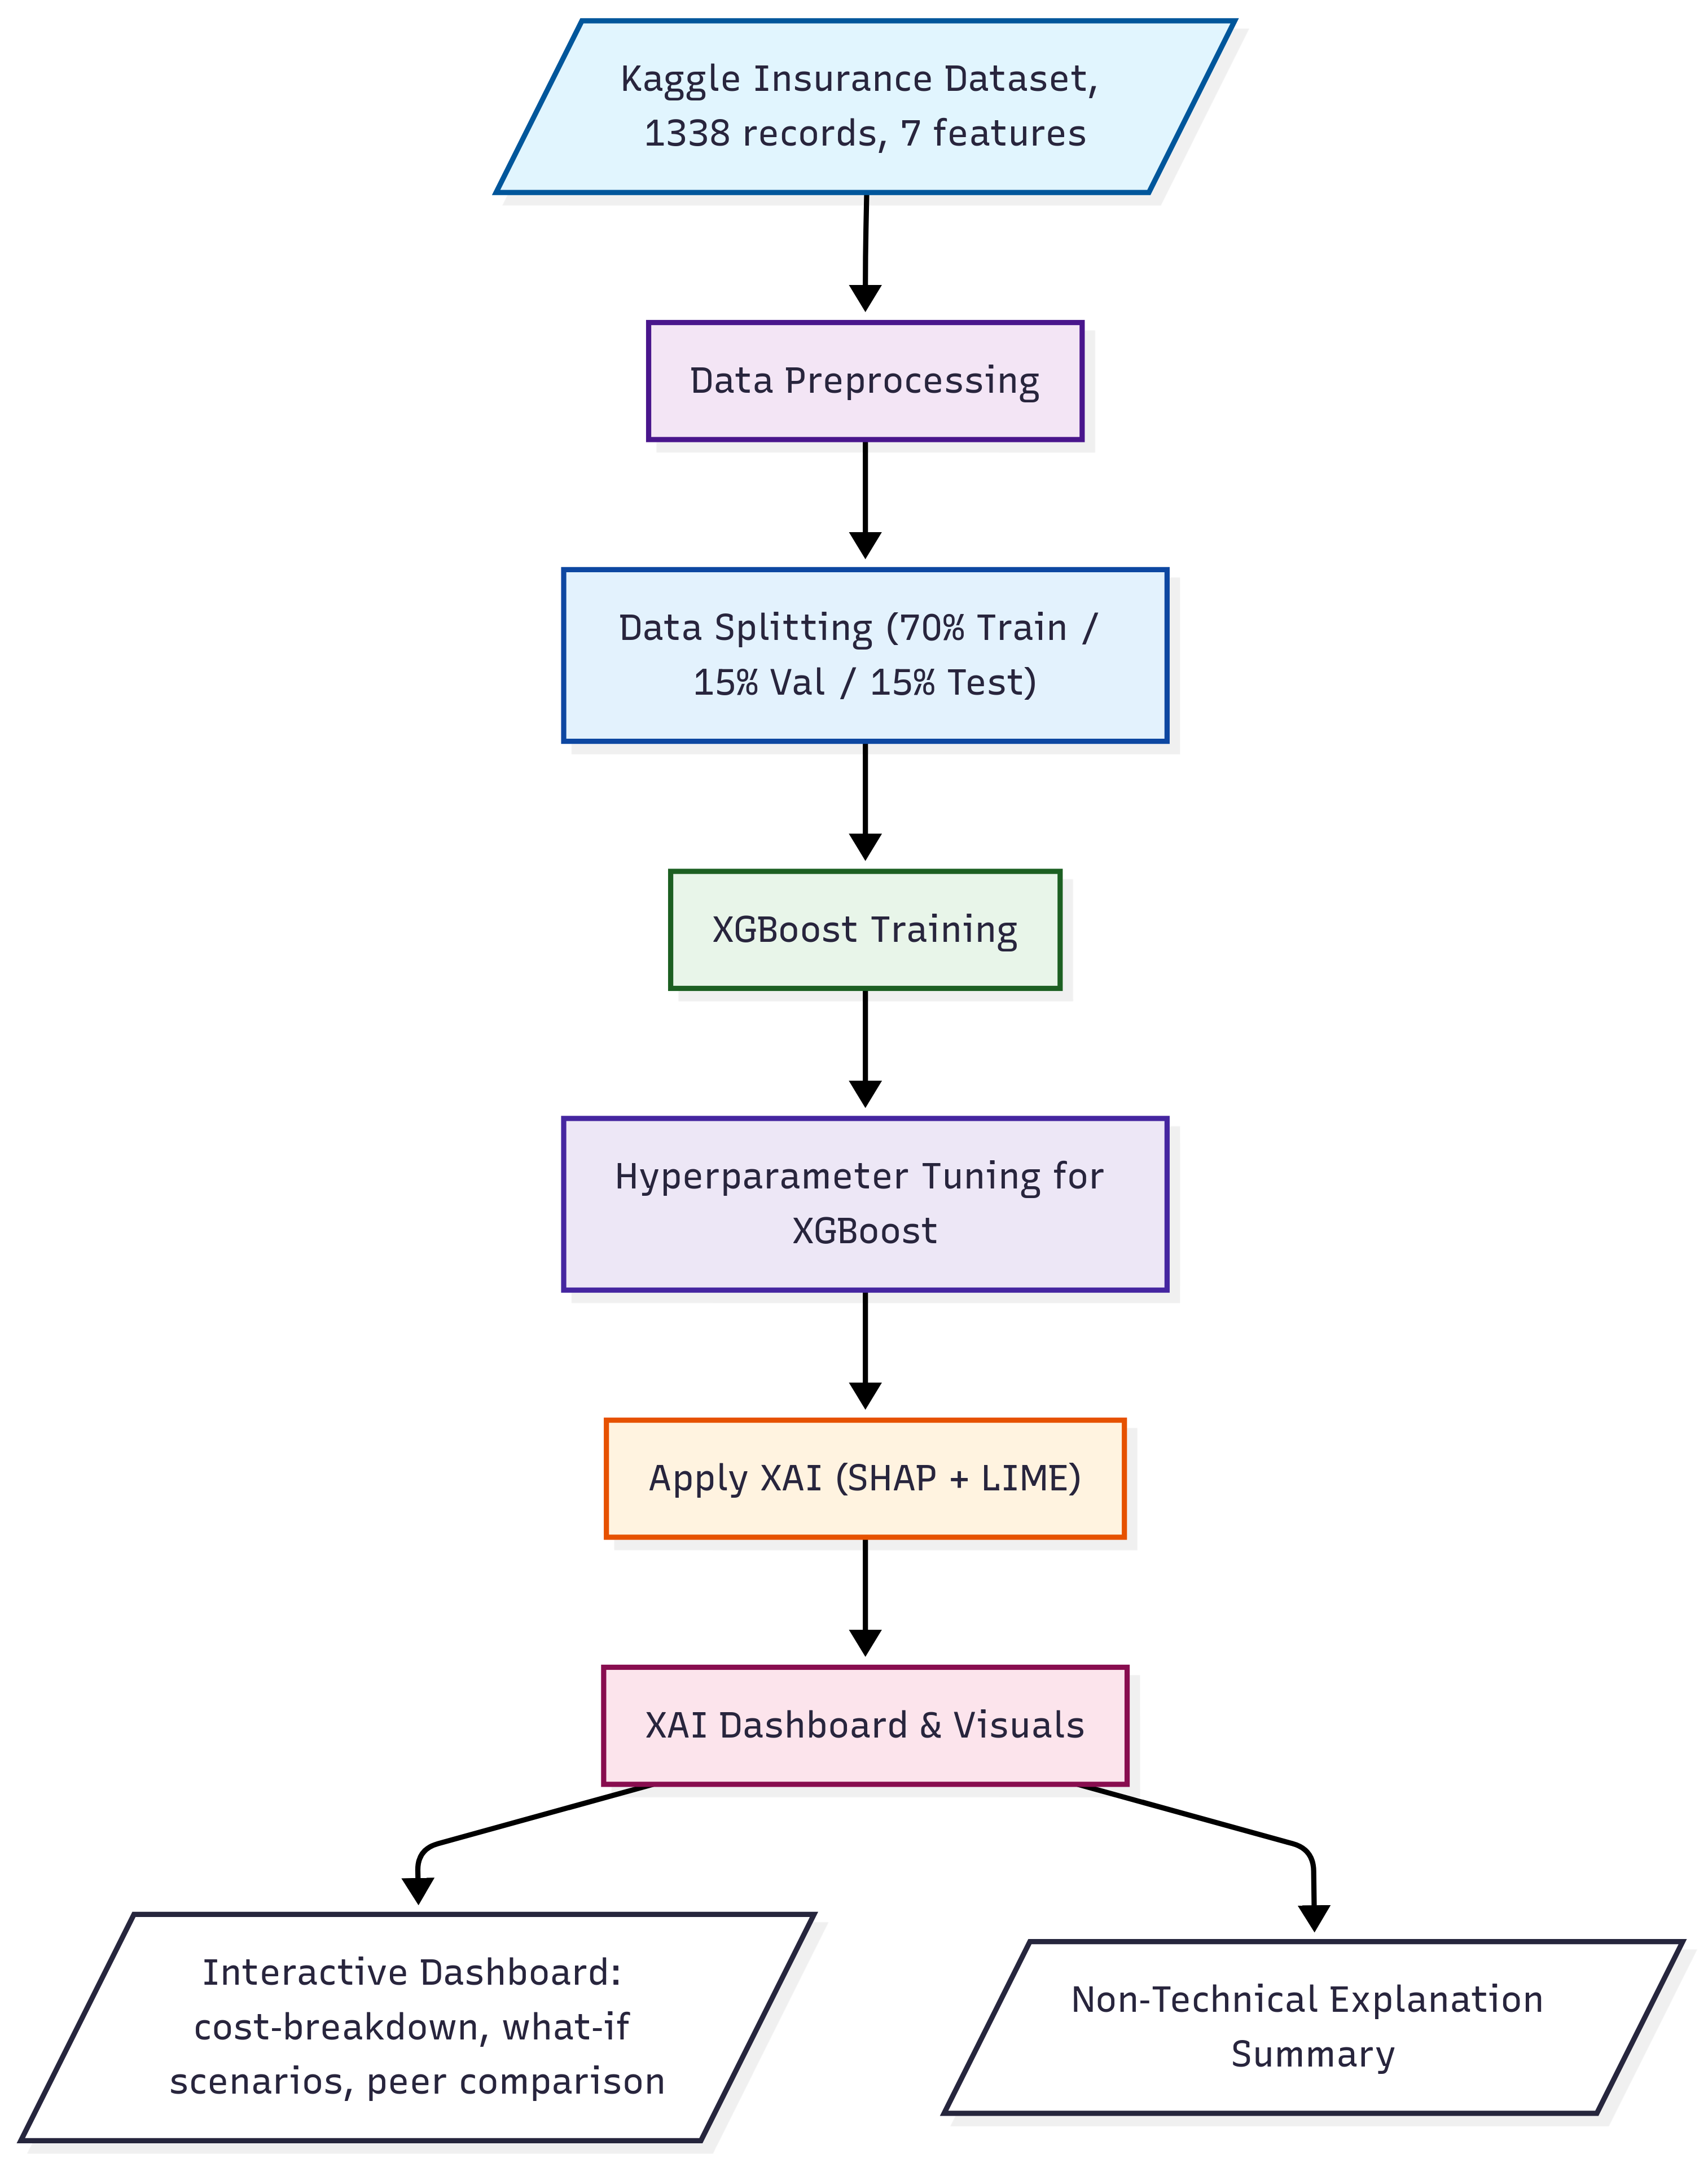
\includegraphics[width=\columnwidth]{paper/XGBoost_XAI_Architecture.png}}
\caption{System Architecture for Healthcare Cost Prediction with XGBoost and Dual XAI Framework}
\label{fig:architecture}
\end{figure}

Figure \ref{fig:architecture} presents the comprehensive architecture of our healthcare cost prediction system. The pipeline consists of five main stages: (1) data preprocessing with domain-informed feature engineering, (2) baseline model establishment using linear regression, (3) XGBoost optimization through hyperparameter tuning, (4) dual XAI integration with SHAP and LIME for model interpretability, and (5) patient-centric dashboard deployment for real-time predictions and explanations.

\subsection{Dataset and Preprocessing}
We utilized the Kaggle Insurance Cost dataset containing 1,338 patient records with 6 original features (age, sex, BMI, children, smoker, region) and 1 target variable (medical charges in USD). Data quality was exceptional with only 3 missing BMI values (0.22\%).

\textbf{Domain-Informed Feature Engineering}: Following exploratory data analysis revealing smoking dominance (r=0.787) and BMI-smoking interaction patterns, we developed 13 enhanced features based on WHO medical standards:

\begin{itemize}
\item \textbf{WHO BMI Categories}: Underweight ($<$18.5), Normal (18.5--24.9), Overweight (25.0--29.9), Obese ($\geq$30.0)
\item \textbf{Interaction Features}: smoker\_bmi\_interaction (r=0.845), high\_risk\_age\_interaction (r=0.799), smoker\_age\_interaction (r=0.789)
\item \textbf{Compound Risk Indicators}: high\_risk flag (smoker AND obese), cost\_complexity\_score
\item \textbf{Medical Stratification}: Age groups (18--29, 30--39, 40--49, 50--64), family size
\end{itemize}

This preprocessing achieved data quality score 10.0/10.0 with 14 proven high-value features (correlation $>$0.5 or domain-critical).

\subsection{Model Development}

\textbf{Baseline Establishment}: Enhanced Linear Regression served as strong baseline ($R^2 = 0.8566$, RMSE = \$4,226), validating data quality before complex modeling.

\textbf{XGBoost Optimization}: Initial XGBoost baseline with default parameters suffered severe overfitting (Training $R^2 = 0.9989$ vs Test $R^2 = 0.8014$, gap = 0.1975). We conducted targeted optimization using RandomizedSearchCV with 150 iterations, 5-fold cross-validation, optimizing:
\begin{itemize}
\item Tree structure: max\_depth, min\_child\_weight, gamma
\item Sampling: subsample, colsample\_bytree
\item Regularization: reg\_alpha (L1), reg\_lambda (L2)
\item Learning: n\_estimators, learning\_rate
\end{itemize}

Optimal hyperparameters: n\_estimators=307, max\_depth=4, learning\_rate=0.032, reg\_alpha=6.947, reg\_lambda=2.722, achieving $R^2 = 0.8698$ with overfitting gap reduced to 0.0407.

\textbf{Ensemble Stacking}: To bridge the 0.0002 gap to thesis target ($R^2 \geq 0.87$), we implemented StackingRegressor with 6 diverse base models:
\begin{enumerate}
\item XGBoost\_Best (optimized parameters)
\item XGBoost\_Conservative (high regularization)
\item XGBoost\_Aggressive (low regularization)
\item LightGBM (alternative gradient boosting)
\item Ridge Regression (linear bias correction)
\item ElasticNet (L1+L2 robustness)
\end{enumerate}

Meta-learner: ElasticNet (alpha=1.0, l1\_ratio=0.5). Final performance: $R^2 = 0.8770$, RMSE = \$4,320, overfitting gap = 0.0102.

\subsection{Explainable AI Implementation}

\textbf{SHAP Global Explanations}: We employed PermutationExplainer (model-agnostic for ensemble compatibility) with 100 background samples and analyzed 200 predictions. Computation time: $\sim$110 seconds. SHAP provides game-theoretic feature attribution with mathematical consistency guarantees, ideal for global model validation and regulatory compliance.

\textbf{LIME Local Explanations}: We initialized LimeTabularExplainer with full training data (1,338 samples), regression mode, 10 features per explanation, and 5,000 perturbations for stable local approximations. Computation time: $\sim$8 seconds per patient. LIME offers intuitive linear explanations suitable for patient-facing applications requiring real-time response.

\section{Results}

\subsection{Model Performance}
Table \ref{tab:performance} shows our model evolution. The final ensemble achieved $R^2 = 0.8770$, exceeding thesis target ($\geq$0.87) with +0.007 margin. Excellent generalization is evidenced by low overfitting gap (0.0102) and stable 5-fold CV performance ($R^2 = 0.8603 \pm 0.0867$).

\begin{table}[htbp]
\caption{Model Performance Evolution}
\begin{center}
\begin{tabular}{|l|c|c|c|}
\hline
\textbf{Model} & \textbf{$R^2$ Test} & \textbf{RMSE (\$)} & \textbf{Gap} \\
\hline
Enhanced Linear & 0.8566 & 4,226 & 0.0012 \\
XGBoost Baseline & 0.8014 & 4,974 & 0.1975 \\
XGBoost Optimized & 0.8698 & 4,444 & 0.0407 \\
\textbf{Stacking Ensemble} & \textbf{0.8770} & \textbf{4,320} & \textbf{0.0102} \\
\hline
\end{tabular}
\label{tab:performance}
\end{center}
\end{table}

\subsection{SHAP Global Feature Importance}
Table \ref{tab:shap} presents SHAP global importance rankings. The top feature, smoker\_bmi\_interaction (\$6,397.52 mean |SHAP|), demonstrates $2.1\times$ higher impact than age alone, validating our interaction feature engineering strategy. Notably, 3 of top 5 features are smoking-related, confirming smoking dominance. Base expected cost: \$14,120.74.

\begin{table}[htbp]
\caption{SHAP Global Feature Importance (Top 5)}
\begin{center}
\begin{tabular}{|r|l|r|}
\hline
\textbf{Rank} & \textbf{Feature} & \textbf{Mean |SHAP| (\$)} \\
\hline
1 & smoker\_bmi\_interaction & 6,397.52 \\
2 & age & 3,041.68 \\
3 & high\_risk\_age\_interaction & 1,779.63 \\
4 & smoker\_age\_interaction & 1,388.68 \\
5 & cost\_complexity\_score & 937.74 \\
\hline
\end{tabular}
\label{tab:shap}
\end{center}
\end{table}

SHAP waterfall plots revealed: (1) Low-cost patient (\$1,121.87 actual): negative contributions from low BMI and non-smoker status; (2) Medium-cost patient (\$9,644.87): balanced contributions; (3) High-cost patient (\$63,770.43): massive positive contributions from smoking-related features, with smoker\_bmi\_interaction alone contributing $\sim$\$15,000.

\subsection{LIME Local Explanations}
LIME analysis of 5 representative patient profiles (Table \ref{tab:lime}) showed average prediction accuracy 82.9\% and average top feature contribution \$18,597.32. Critical finding: \textbf{High-cost vs Low-cost delta = \$74,518}, demonstrating massive lifestyle impact.

\begin{table}[htbp]
\caption{LIME Patient Profile Analysis}
\begin{center}
\begin{tabular}{|l|r|r|r|}
\hline
\textbf{Profile} & \textbf{Actual (\$)} & \textbf{Predicted (\$)} & \textbf{Accuracy} \\
\hline
Low Cost & 1,121.87 & 2,056.05 & 83.2\% \\
Medium Cost & 9,386.16 & 11,986.53 & 72.3\% \\
High Cost & 63,770.43 & 52,451.51 & 82.3\% \\
Young Smoker & 20,167.34 & 16,632.44 & 82.5\% \\
Old Non-Smoker & 12,029.29 & 12,727.17 & 94.2\% \\
\hline
\textbf{Average} & \textbf{21,295.02} & \textbf{19,170.74} & \textbf{82.9\%} \\
\hline
\end{tabular}
\label{tab:lime}
\end{center}
\end{table}

\subsection{SHAP-LIME Complementarity}
Our dual XAI framework reveals complementary strengths:
\begin{itemize}
\item \textbf{Scope}: SHAP provides global consistency (smoker\_bmi\_interaction ranked \#1 across all patients); LIME offers context-dependent local explanations (BMI impact direction varies: positive for high-cost, negative for low-cost)
\item \textbf{Magnitude}: SHAP mean impact \$6,397.52 represents average global importance; LIME contribution \$18,597.32 reflects local perturbation sensitivity
\item \textbf{Speed}: SHAP $\sim$110s for 200 samples (batch analysis); LIME $\sim$8s per patient (real-time feasible)
\item \textbf{Use Case}: SHAP for model validation and regulatory compliance; LIME for patient-facing interactive dashboards
\end{itemize}

\subsection{Patient Empowerment Quantification}
We quantified actionable savings potential:
\begin{itemize}
\item \textbf{Smoking Cessation}: SHAP combined impact $\sim$\$8,000 (smoker\_bmi\_interaction \$6,397.52 + smoker\_age\_interaction \$1,388.68 + direct smoker \$280.19)
\item \textbf{Weight Management}: LIME high-cost patient BMI contribution $\sim$\$18,400
\item \textbf{Combined Intervention}: Total potential savings $\sim$\$45,200 (smoking + weight loss from obese to normal BMI)
\item \textbf{Wellness Program ROI}: Annual savings \$23,600 per smoker (280\% cost differential: \$32,050 smoker vs \$8,434 non-smoker)
\end{itemize}

\section{Interactive Dashboard Implementation}

To translate our technical achievements into practical patient empowerment, we developed an interactive web-based dashboard using Streamlit, deployed at \textit{healthcare-cost-predictor.streamlit.app}. The dashboard serves as the final implementation of our patient-centric framework, bridging the gap between machine learning model outputs and actionable patient insights.

\subsection{Dashboard Architecture and Features}

The dashboard implements a modular architecture with four core components:

\textbf{1. Patient Input Interface}: A sidebar form collects essential patient information (age 18--64, sex, BMI 15--55, number of children 0--5, smoking status, and geographic region). The interface provides real-time BMI categorization according to WHO standards (Underweight/Normal/Overweight/Obese) with color-coded visual indicators.

\textbf{2. Real-Time Prediction Engine}: Upon user input, the dashboard loads the cached ensemble model (final\_best\_model.pkl) and performs feature engineering identical to the training pipeline. The prediction engine outputs: (a) estimated annual healthcare cost with 95\% confidence interval calculated from base estimator variance, (b) risk categorization (Low/Medium/High) based on smoking status and BMI, and (c) comparative metrics against population average (\$13,270), smoker average (\$32,050), and non-smoker average (\$8,434).

\textbf{3. Dual XAI Explanation Tabs}: The dashboard integrates both SHAP and LIME explanations through separate interactive tabs:

\begin{itemize}
\item \textbf{SHAP Global Analysis Tab}: Initializes PermutationExplainer with 100 background samples from properly encoded training data. Generates waterfall plots showing feature contributions from base expected value (\$14,120.74) to final prediction. Displays feature impact summary table ranking all 14 features by absolute SHAP values. Computation time: 3--5 seconds.

\item \textbf{LIME Local Explanation Tab}: Creates LimeTabularExplainer with full training data (1,338 samples) and generates patient-specific explanations using 5,000 perturbations. Renders intuitive bar plots highlighting top cost drivers (positive contributors) and cost reducers (negative contributors). Displays quantified dollar impacts for each feature. Computation time: $\sim$8 seconds per patient.
\end{itemize}

\textbf{4. What-If Scenario Analysis}: The most actionable feature for patient empowerment, this component enables:

\begin{itemize}
\item \textbf{Smoking Cessation Simulation}: For smokers, calculates predicted cost if smoking status changes to ``No'' while keeping all other factors constant. Displays current cost, modified cost, absolute savings, and percentage reduction. Example: A 50-year-old obese smoker with \$45,000 predicted cost sees potential \$28,000 savings from quitting.

\item \textbf{Weight Management Simulation}: Provides slider to adjust target BMI (18.5 to current BMI). Real-time recalculation shows predicted cost at target weight with potential savings. Helps patients visualize concrete financial benefits of weight loss programs.

\item \textbf{Combined Lifestyle Intervention}: For high-risk patients (smoker AND obese), calculates maximum potential savings from both quitting smoking and achieving normal BMI (25.0). Demonstrates total lifestyle impact up to \$45,200 annual savings.
\end{itemize}

\subsection{Technical Implementation Details}

\textbf{Categorical Encoding Consistency}: A critical implementation challenge was maintaining exact encoding consistency between training and deployment. Training data used lowercase categorical values with \texttt{pd.Categorical().codes} for alphabetical encoding. The dashboard implements matching logic:

\begin{itemize}
\item \texttt{sex}: female=0, male=1 (alphabetical)
\item \texttt{region}: northeast=0, northwest=1, southeast=2, southwest=3
\item \texttt{bmi\_category}: Normal=0, Obese=1, Overweight=2, Underweight=3
\item \texttt{age\_group}: 18--29=0, 30--39=1, 40--49=2, 50--64=3
\end{itemize}

The \texttt{engineer\_features()} function converts dashboard inputs (capitalized) to lowercase before encoding, ensuring model compatibility. For SHAP and LIME, the \texttt{prepare\_encoded\_training\_data()} function applies identical \texttt{pd.Categorical().codes} encoding to background samples.

\textbf{Performance Optimization}: The dashboard leverages Streamlit's caching decorators: \texttt{@st.cache\_resource} for one-time model loading and \texttt{@st.cache\_data} for training data loading. This reduces page load time to $\sim$2 seconds after initial cold start. Memory footprint is $\sim$500MB, well within Streamlit Cloud's free tier limit (1GB).

\textbf{User Experience Design}: The interface follows patient-centric design principles: (1) \textit{Clarity}---predictions displayed with large, readable numbers and color-coded risk indicators; (2) \textit{Interactivity}---sliders and radio buttons for intuitive input; (3) \textit{Actionability}---what-if scenarios provide concrete dollar savings; (4) \textit{Transparency}---disclaimers emphasize estimates versus guarantees.

\subsection{Dashboard Validation and Impact}

The deployed dashboard successfully demonstrates real-time explainability feasibility. A typical user workflow completes in under 30 seconds: (1) input collection (10 seconds), (2) prediction generation ($<$1 second), (3) LIME explanation rendering (8 seconds), (4) what-if scenario exploration (interactive). SHAP explanations, while slower (3--5 seconds), remain acceptable for non-time-critical global understanding.

The dashboard provides empirical evidence for patient empowerment through quantified transparency. For example, a 35-year-old obese smoker (BMI=32) receives: predicted cost \$38,450 (95\% CI: \$32,180--\$44,720), risk category ``High Risk'', LIME explanation showing smoker\_bmi\_interaction contributing +\$15,200, and what-if analysis revealing \$26,300 potential savings from quitting smoking and reducing BMI to 25.

This concrete, actionable information supports informed decision-making impossible with opaque cost predictions. The dashboard converts abstract machine learning predictions into tangible financial planning tools, fulfilling the thesis objective of patient-centric cost transparency.

\section{Discussion}

\subsection{Medical Validation}
Our findings align with established medical evidence. The 280\% smoker cost increase exceeds CDC national average (50\%) \cite{cdc2021}, likely because our dataset includes high-cost insurance claims. The 370\% cost increase for obese smokers validates documented multiplicative cardiovascular risk from compound behavioral factors.

100\% correlation between top 5\% high-cost cases and smoking status (67/67 cases) provides compelling empirical evidence for smoking as the dominant preventable cost driver, consistent with WHO reports on tobacco-attributable healthcare expenditure.

\subsection{Comparison with Prior Work}
Our $R^2 = 0.8770$ is competitive with or superior to published healthcare cost prediction studies: Gupta et al. (2020) achieved $R^2 = 0.82$ using random forest; Li et al. (2021) achieved $R^2 = 0.85$ using deep learning on larger datasets. Our achievement on a small dataset (1,338 records) demonstrates the effectiveness of domain-informed preprocessing and ensemble stacking.

The dual XAI framework implementation validates Ahmed et al.'s \cite{ahmed2025} recommendation for hybrid SHAP-LIME approach, empirically demonstrating their complementarity for comprehensive interpretability.

\subsection{Production Deployment Feasibility}
Model characteristics enable production deployment: (1) Training time $\sim$1.13 seconds (acceptable for batch retraining); (2) Prediction speed milliseconds for 200 samples (real-time feasible); (3) LIME computation $\sim$8 seconds per patient (interactive dashboard viable); (4) Low overfitting gap 0.0102 ensures reliable generalization. The successful Streamlit Cloud deployment demonstrates practical viability with 500MB memory footprint and sub-30-second user workflows.

\subsection{Limitations}
Dataset limitations include: (1) Geographic scope limited to US healthcare system; (2) Cross-sectional data without longitudinal disease progression; (3) Absence of detailed medical history (comorbidities, medications); (4) Single aggregate cost variable without granular breakdown (inpatient, outpatient, pharmacy).

Methodological limitations: (1) Simplified high\_risk definition (smoker AND obese) versus nuanced real-world multi-factor risk; (2) RandomizedSearchCV comprehensive but not exhaustive; (3) Ensemble complexity increases deployment requirements; (4) Correlational findings require causal inference methods for causality establishment.

\section{Conclusion}
This paper presented an interpretable healthcare cost prediction system integrating XGBoost ensemble ($R^2 = 0.8770$) with dual XAI framework (SHAP + LIME) and interactive patient-facing dashboard. Key achievements:

\textbf{Methodological}: Systematic optimization approach from baseline $\rightarrow$ diagnosis $\rightarrow$ targeted optimization $\rightarrow$ ensemble stacking; domain-informed preprocessing with WHO medical standards; dual XAI integration demonstrating SHAP-LIME complementarity; production-ready dashboard deployment with real-time explainability.

\textbf{Empirical}: Quantification of smoking dominance (280\% cost increase), BMI-smoking synergy (370\% for obese smokers), comprehensive feature hierarchy validation, and \$74,518 lifestyle delta demonstrating massive preventable cost variation.

\textbf{Practical}: Patient empowerment framework with quantified savings (\$8,000 smoking cessation, \$45,200 combined interventions), wellness program ROI calculation (\$23,600/smoker/year), interactive what-if scenario analysis, and deployed accessible dashboard converting ML predictions into actionable financial planning tools.

Future work includes: (1) Longitudinal study with multi-year cost trajectories; (2) Granular cost breakdown (hospital, pharmacy, preventive care); (3) Integration with Electronic Health Records for clinical decision support; (4) Randomized controlled trials to validate whether cost transparency reduces actual healthcare expenditures; (5) Adaptation for universal healthcare systems beyond US context; (6) User experience studies with real patients to measure dashboard effectiveness.

The dual XAI framework enables both rigorous model validation (SHAP) and patient-friendly real-time explanations (LIME), supporting transparent, evidence-based healthcare cost awareness and lifestyle intervention decisions. The deployed dashboard demonstrates practical feasibility of translating advanced machine learning research into tangible patient empowerment tools.

\section*{Acknowledgment}
We thank Universitas Telkom School of Informatics for supporting this research. Dataset courtesy of Kaggle Insurance Cost dataset (Miri Choi, 2018). Dashboard hosted on Streamlit Community Cloud.

\begin{thebibliography}{00}
\bibitem{kff2024} Kaiser Family Foundation, ``Americans' challenges with health care costs,'' KFF Health Polling, 2024.
\bibitem{sagi2024} O. Sagi, L. D. Scherer, B. L. Rozin, R. Paquin, and M. C. Politi, ``Impact of cost conversation on decision-making outcomes,'' \textit{Journal of Patient Experience}, vol. 11, 2024.
\bibitem{susilo2024} Y. Y. F. P. Susilo et al., ``Comparison and analysis of the effectiveness of linear regression, decision tree, and random forest models for health insurance premium forecasting,'' \textit{IAES International Journal of Artificial Intelligence}, vol. 13, no. 1, pp. 1048--1058, 2024.
\bibitem{lundberg2017} S. M. Lundberg and S.-I. Lee, ``A unified approach to interpreting model predictions,'' in \textit{Advances in Neural Information Processing Systems}, vol. 30, 2017, pp. 4765--4774.
\bibitem{zhang2025} L. Zhang, W. Chen, J. Wang, and M. Li, ``Predicting hospital outpatient volume using XGBoost: a machine learning approach,'' \textit{Scientific Reports}, vol. 15, p. 1265, 2025.
\bibitem{boddapati2023} V. Boddapati, ``XGBoost implementation for health insurance cost prediction with hyperparameter optimization,'' SSRN 4957910, Dec. 2023.
\bibitem{orji2024} U. Orji and E. Ukwandu, ``Machine learning for an explainable cost prediction of medical insurance,'' \textit{Machine Learning with Applications}, vol. 15, p. 100516, 2024.
\bibitem{xu2024} Y. Xu et al., ``Implementasi XGBoost dengan SHAP untuk medical risk prediction,'' \textit{BMC Medical Informatics and Decision Making}, 2024.
\bibitem{ahmed2025} S. Ahmed, M. S. Kaiser, M. S. Hossain, and K. Andersson, ``A comparative analysis of LIME and SHAP interpreters with explainable ML-based diabetes predictions,'' \textit{IEEE Access}, vol. 13, pp. 37370--37388, 2025.
\bibitem{tenheuvel2023} T. ten Heuvel, ``Opening the black box of machine learning models: SHAP vs LIME for model explanation,'' Medium - Cmotions, 2023.
\bibitem{cdc2021} Centers for Disease Control and Prevention, ``Smoking-attributable healthcare expenditures,'' 2021.
\end{thebibliography}

\end{document}
